\documentclass[12pt]{article}
\usepackage[whole]{bxcjkjatype}
\usepackage{epsf}
\usepackage{amsmath,amssymb}
\usepackage{bm}

\usepackage{graphicx}

\usepackage{comment}
\usepackage{multirow}
\usepackage{braket}

\usepackage{hyperref}
\usepackage{tgtermes}
\usepackage{float}
\usepackage{xcolor}
\usepackage{siunitx}
\usepackage{mhchem}
\usepackage{cite}

\usepackage{cleveref}

% set margin
\usepackage[margin=1in]{geometry}

% remove the page number
% \pagestyle{empty}

% set section title all caps
\usepackage{titlesec}
\titleformat*{\section}{\large\bf}
\titleformat*{\subsection}{\normalsize\bf}
\titlespacing*{\section}{0pt}{1.6em}{1em}
\titlespacing*{\subsection}{0pt}{1.6em}{1em}

% publications title
\renewcommand{\refname}{References}

% base line stretch
\renewcommand{\baselinestretch}{1.1}
\allowdisplaybreaks[1]


% customize the title
\usepackage{titling}
\pretitle{\vspace{-1in}}
\title{{\Large Research Statement}}
\posttitle{
  \par
}
\preauthor{\vspace{0.5em}}
\author{
  \indent{\large So Chigusa}\\
  \indent\textit{schigusa@mit.edu}\\
  \indent\textit{Massachusetts Institute of Technology, 77 Massachusetts Avenue, Cambridge, MA 02139}
}
\postauthor{}
\date{\vspace{-3em}}

\begin{document}
\maketitle

My research area lies at the intersection of quantum science and theoretical particle physics.
The rapid advancement of quantum science technologies is continuously introducing new solutions to problems.
These include \textbf{quantum metrology} techniques for detecting faint signals and \textbf{quantum computation} for simulating dynamics by directly manipulating quantum states.
In light of this, I believe it crucial to explore how these advancements can be used to investigate physics.
With this in mind, I am researching: \textit{(i) direct detection of light dark matter using quantum metrology}, and \textit{(ii) quantum algorithms to simulate parton shower dynamics}.

\subsection*{Direct detection of light dark matter using quantum metrology}

One of my research areas focuses on developing methods to explore \textbf{light dark matter} using quantum metrology techniques.
Conventional dark matter direct detection programs, which primarily focus on the $\mathrm{GeV}$-mass region, have yet to provide any evidence of dark matter.
This has motivated the community to explore a broader mass range, including the sub-$\mathrm{GeV}$ scale, which remains largely unexplored, in part due to the challenges like low excitation energy and small event rates.
Quantum metrology techniques offer promising ways for detecting such faint signals.
By leveraging these advanced techniques, I aim to overcome current limitations in sensitivity and frequency coverage, paving the way for new approaches in light dark matter search.

Among light dark matter candidates, I primarily focus on a pseudo-scalar candidate often referred to as \textbf{axion dark matter}, which is strongly motivated from a high-energy theoretical perspective.
The axion provides a compelling solution to the puzzle of conserved CP symmetry in the strong interaction sector.
It can also naturally emerge from an ultraviolet completion of the theory including gravity, the string theory.
From a metrological perspective, the axion is particularly intriguing because its interaction with ordinary fields mimics electromagnetic fields while exhibiting several distinctive features that allow it to be distinguished from conventional electromagnetic fields.
These features include a spin-dependent coupling strength entirely uncorrelated with the gyromagnetic ratio and a signal coherence time directly correlated with its frequency.
In this context, my research aims to develop quantum metrology protocols that fully exploit these distinctive characteristics of the axion dark matter signal to maximize its detection potential.
In \cref{fig:summary}, I provide a summary plot illustrating the frequency coverage of various approaches I have investigated.
Below, I will detail these approaches with reference to this figure.

\begin{figure}[t]
  \centering
  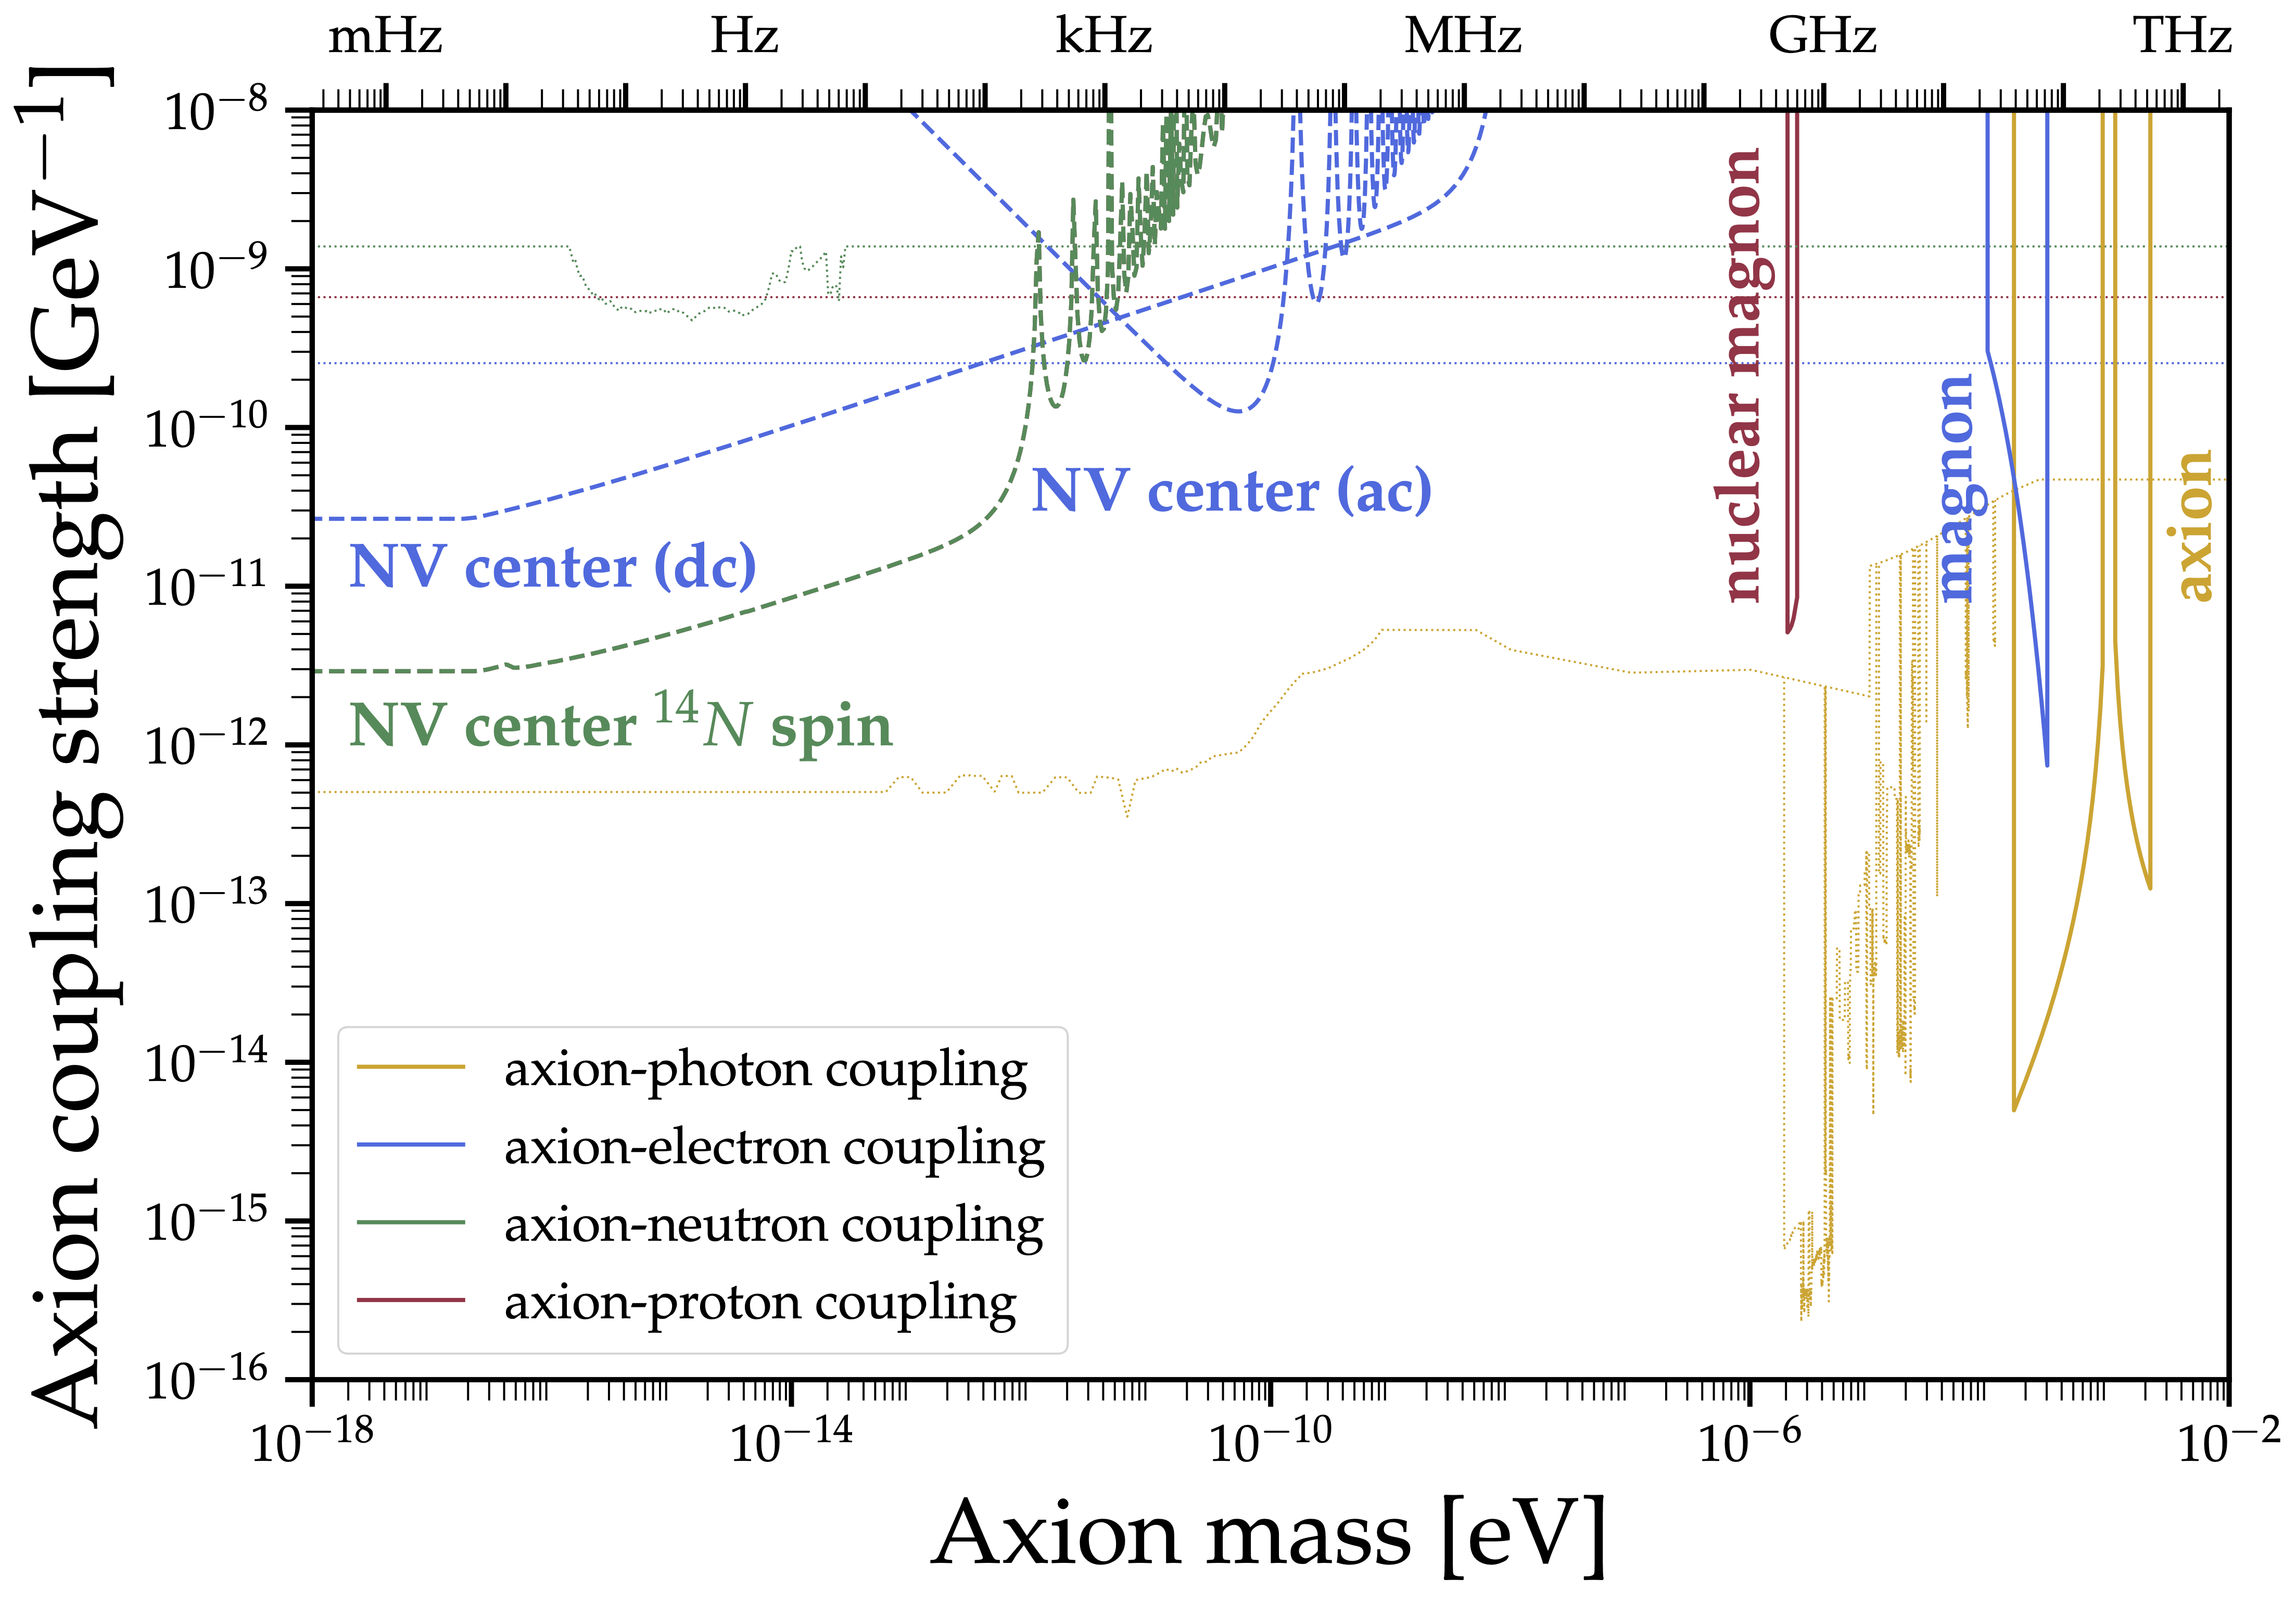
\includegraphics[width=0.8\hsize]{../public/rs/Summary_Plot_2024.png}
  \caption{
    Summary of the frequency coverage of various approaches discussed in the main text.
    The prospects for the pseudo-scalar (axion) dark matter are shown for the purpose of demonstration.
    Each result, represented by a solid or dashed line, should be compared with the current constraint, which is plotted as a dashed line of the same color corresponding to the same coupling.
  }
  \label{fig:summary}
\end{figure}

I have explored three distinct approaches utilizing different collective excitations of spins: \textbf{magnon} \cite{Chigusa:2020gfs}, \textbf{axion} \cite{Chigusa:2021mci}, and \textbf{nuclear magnon} \cite{Chigusa:2023hmz}, each probing different dark matter couplings.
The frequency coverage of these approaches is shown by solid lines in \cref{fig:summary}.
If the dark matter mass lies in the challenging sub-$\mathrm{THz}$ range, approaches using these excitations provide one of the few valuable detection opportunities.
Many ongoing experiments, including QUAX and TOORAD experiments, are currently searching for spin excitations with similar concepts, which may ultimately lead to the discovery of dark matter.

In Refs. \cite{Chigusa:2023hms}, \cite{Chigusa:2024psk}, I proposed a light dark matter search using \textbf{nitrogen-vacancy center} magnetometry.
This specialized quantum metrology technique aids in developing new approaches with broad frequency coverage and/or improved sensitivity, which are briefly summarized in dashed lines in \cref{fig:summary}.
My approach leverages the sensitivity of nitrogen-vacancy centers to various spin species, clearly shown by different colors of dashed lines, and offers a novel way to distinguish magnetic noise from dark matter signals.
Recently, we launched an experiment based on these ideas at the International Center for Quantum-field Measurement Systems for Studies of the Universe and Particles (QUP).
This experimental collaboration has published a paper on a data analysis method for incoherent signals \cite{10.1063/5.0223678}, motivated by dark matter, and is now moving towards cryogenic experimental operation.

Among the quantum techniques designed to surpass the standard quantum limit and approach the Heisenberg limit, I focus on \textbf{squeezing} and \textbf{entanglement}.
I explored the possibility of enhancing the nuclear magnon signal excited in superfluid $\mathrm{^3He}$ through squeezing and identified conditions where this improves sensitivity \cite{Chigusa:2023szl}.
These conditions must be carefully examined to assess the potential of squeezing for spin-based dark matter searches, including \cite{Chigusa:2020gfs}, \cite{Chigusa:2021mci}, \cite{Chigusa:2023hmz}, where the signal coherence time is limited.
Regarding entanglement, while certain entangled states, such as the \textbf{Greenberger–Horne–Zeilinger state}, are known as a way to achieve the Heisenberg limit, they are often vulnerable to Markovian noise, negating the advantage of entanglement.
I investigated this issue in the context of dark matter searches \cite{Sichanugrist:2024wfk}, identifying situations where entangled states can enhance sensitivity even in the presence of noise, leaving further optimization as a future direction.

My future project plans involve the continued development of metrology techniques to expand their applicability to new physics.
I intend to develop metrology techniques that integrate \textbf{error correction} and \textbf{quantum correlation}, extensively studied in particular in the context of quantum computation and clock synchronization, to enhance sensitivity to signals with multiple unknown properties.
Additionally, building on the methodologies developed for light dark matter detection, I plan to apply similar concepts to other targets, such as \textbf{high-frequency gravitational waves} and the \textbf{cosmic axion background}.
These efforts will position my research to contribute significantly to the broader field of quantum metrology and its applications in uncovering new physics.

\subsection*{Quantum algorithms to simulate parton shower dynamics}

\begin{figure}[t]
  \centering
  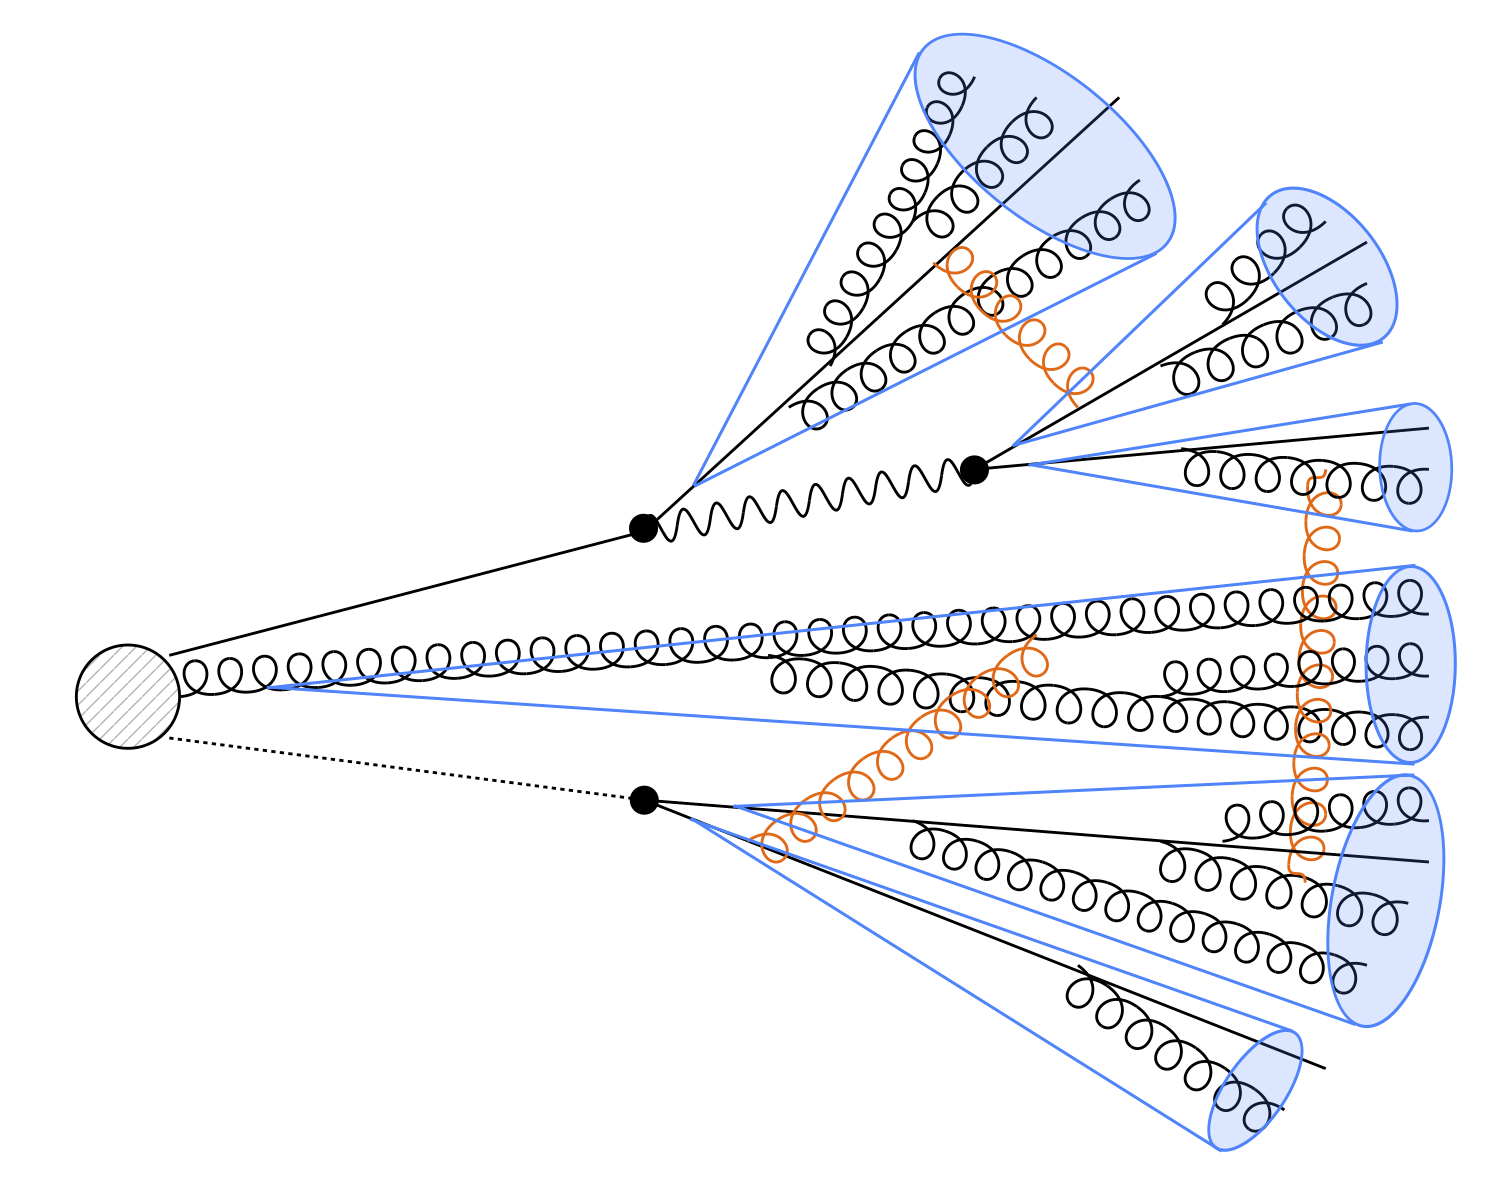
\includegraphics[width=0.6\hsize]{../public/rs/shower_annotated.png}
  \caption{
    A schematic illustration of a multi-emission process that incorporates quantum interference effects beyond the classical parton shower treatment.
    The leading-order contribution to inclusive parton shower dynamics is fully captured by blue cones, which represent collinear emissions and can be treated independently.
    At the next-to-leading order, however, soft interference effects, depicted by orange lines in the figure, must be considered, potentially leading to global event-wise entanglement.
  }
  \label{fig:shower}
\end{figure}

Another direction of my research focuses on developing quantum algorithms to study quantum dynamics.
Today, quantum computing resources with a substantial number of qubits are publicly accessible, and their availability is steadily increasing.
Given this, now is the ideal time to explore quantum algorithms for physics research.
Leveraging this opportunity, my research aims to push the boundaries of quantum simulations to better understand complex physical systems.

As an important example of systems with intriguing quantum properties, I work on \textbf{parton showers}.
The original parton shower algorithm is a classical approach that has been widely used for multi-emission processes (see \cref{fig:shower} for a schematic illustration) in collider and astroparticle physics.
However, it fails to incorporate important \textbf{quantum interference effects}, which can significantly alter the particle multiplicity distribution, especially in the presence of a non-trivial flavor structure \cite{Chigusa:2022act}.
To address this issue, I developed a \textbf{quantum parton shower algorithm} using a veto procedure \cite{Bauer:2023ujy}, which can incorporate the exponentially growing number of diagrams while utilizing polynomial quantum resources.
This is the first quantum algorithm capable of reconstructing full kinematic information, making an important first step towards realistic quantum simulations of parton shower dynamics.

I plan to further develop quantum algorithms addressing both computational and physical aspects.
The sampling method for the evolution variable, the virtuality, can be optimized to reduce the gate cost, although it distorts quantum states due to the artificial veto procedure.
I am developing an algorithm to restore the correct quantum state with an improved sampling method.
Additionally, I intend to develop algorithms that incorporate next-to-leading order effects, extending beyond the collinear emissions represented by blue cones in \cref{fig:shower}.
To achieve this, \textbf{soft interference effects} must be properly accounted for by storing the emission history in qubits.
This approach fully leverages the advantages of quantum computing because of the possibility of global event-wise entanglement, illustrated by the orange lines in \cref{fig:shower} that connect the blue cones.
By developing these algorithms, I aim to create a comprehensive toolkit for quantum simulations of scattering processes at high-energy colliders, properly incorporating quantum interference effects.

\subsection*{Conclusion}

The program for exploring new physics should evolve alongside rapid technological advancements of quantum science.
By incorporating advanced quantum metrology techniques and developing quantum algorithms, I aim to develop innovative approaches for exploring physics with the ultimate goal of contributing to a deeper understanding of the universe's fundamental mysteries.

\bibliographystyle{JHEP}
\bibliography{publications.bib}

\end{document}
